\documentclass[10pt,letterpaper]{article}
\usepackage[utf8]{inputenc}
\usepackage{amsmath}
\usepackage{amsfonts}
\usepackage{amssymb}
\usepackage{graphicx}
\usepackage[letterpaper]{geometry}
\usepackage{hyperref}
\geometry{verbose,tmargin=1in,bmargin=1in,lmargin=1in,rmargin=1in}
\setlength{\parskip}{\medskipamount}
\setlength{\parindent}{0pt}

%\usepackage{babel}


\author{Mudasar Zahoor}
\date{}

\begin{document}

\title{Non-Hardening Von-Mises Plasticity}
\maketitle


This write-up gives details for the single element (affine) plasticity verification test for transient stress eigenvlaues with stationary eigenvectors \cite{kamojjala2015}.

\section{Statement}
\begin{itemize}
\item Piecewise constant strain rate problem resulting in rotation of deviatoric
stress
\item For Von-Mises plasticity, deviatoric stress is constant. Therefore,
the rotation of the stress deviator is actually motion on a sphere
embedded in the five-dimensional space of deviatoric symmetric tensors.
\item The stress moves along a circumference of the sphere to align itself
toward the constant applied strain rate deviator.
\item The angle between the strain rate and stress deviator decays exponentially
to zero.
\end{itemize}

\section{Time Varying Solution}

For $t>t_{0}$($t_{0}$ is the start time of the time varying part) \cite{Brannon_2}:
\begin{itemize}
\item Unit Tensor in the direction of deviatoric stress
\end{itemize}
\[
\underline{N}\left(t\right)=\frac{\left(T-1\right)\underline{E}_{1}+\left(2\sqrt{T}\right)\underline{E}_{2}}{T+1}
\]

\begin{itemize}
\item Deviatoric Stress
\end{itemize}
\[
\underline{\sigma}^{D}\left(t\right)=\sqrt{2}\tau_{y}\underline{N}\left(t\right)
\]

\begin{itemize}
\item Mean Stress
\end{itemize}
\[
p\left(t\right)=p_{0}+K\dot{\varepsilon_{v}}\left(t-t_{0}\right)
\]

\begin{itemize}
\item Stress
\end{itemize}
\[
\underline{\sigma}\left(t\right)=\underline{\sigma}^{D}\left(t\right)+p\left(t\right)\underline{I}
\]


where,

$T\left(t\right)=\frac{1+n_{01}}{1-n_{01}}e^{\left[\frac{2\dot{\gamma}\left(t-t_{0}\right)}{\alpha}\right]}$;
$n_{01}=\underline{N}_{0}:\underline{E}_{1}$

$\underline{E}_{1}=\frac{\dot{\underline{\gamma}}}{\dot{\gamma}}$

$\underline{E}_{2}=\frac{\underline{N}_{0}-\left(n_{01}\right)\underline{E}_{1}}{\sqrt{1-\left(n_{01}\right)^{2}}}$

$\underline{N}_{0}=\frac{\underline{\sigma}_{0}^{D}}{\sqrt{2}\tau_{y}}$

$\dot{\gamma}=\left\Vert \dot{\underline{\gamma}}\right\Vert =\sqrt{\dot{\gamma}_{ij}\dot{\gamma}_{ij}}$

$\alpha=\frac{\sqrt{2}\tau_{y}}{2G}$

Figure \ref{fig:vm_plast} \cite{brannon2010multi} shows the deviatoric stress space with $\underline{E}_{1}$ as unit tensor in the direction of the strain rate deviator ($\dot{\underline{\gamma}}$). $\underline{E}_{2}$ is a unit tensor orthogonal to $\underline{E}_{1}$. $\underline{N}_{0}$ is a unit tensor in the direction of the initial stress deviator.

\begin{figure}[h]
\noindent \begin{centering}
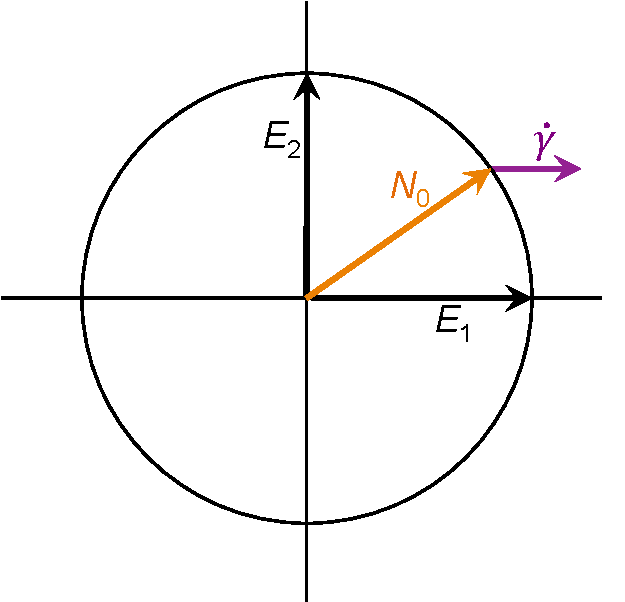
\includegraphics[width=5in]{Affine_Plasticity_Fig}
\par\end{centering}

\caption{Von Mises Plasticity under a constant strain rate. \label{fig:vm_plast}}
\end{figure}

\section{Affine Plasticity test for transient stress eigenvlaues with stationary
eigenvectors}

The exact solution presented above is applicable to non-hardening
Von-Mises plasticity for any constant strain rate that is not aligned
to the yield normal. The solution stands even when the constant strain
rate has time varying principal directions.

Consider a simple piecewise linear strain applied as shown in Table \ref{tab:Strains}.

\begin{table}[h]
\noindent \begin{centering}
\begin{tabular}{|c|c|c|c|}
\hline
time (s) & $\varepsilon_{11}$ & $\varepsilon_{22}$ & $\varepsilon_{33}$\tabularnewline
\hline
\hline
0 & 0 & 0 & 0\tabularnewline
\hline
1 & -0.003 & -0.003 & 0.006\tabularnewline
\hline
2 & -0.0103923 & 0 & 0.0103923\tabularnewline
\hline
\end{tabular}
\par\end{centering}

\caption{Strains\label{tab:Strains}}
\end{table}


The yield in shear is, $\tau_{y}=165MPa$.

The shear modulus is, $G=79000MPa$.


\subsection{Part I: Initial Loading}

During the initial loading, the strain rate is, $\dot{\underline{\gamma}}$:

\[
\dot{\underline{\gamma}}=\left[\begin{array}{ccc}
-0.003 & 0 & 0\\
0 & -0.003 & 0\\
0 & 0 & 0.006
\end{array}\right]
\]


Then, the deviatoric stress rate is, $\dot{\underline{\sigma}}^{D}=2G\dot{\underline{\gamma}}$:

\[
\dot{\underline{\sigma}}^{D}=\left[\begin{array}{ccc}
-474 & 0 & 0\\
0 & -474 & 0\\
0 & 0 & 948
\end{array}\right]
\]


Integrating this constant stress rate over time:

\[
\underline{\sigma}^{D}=\left[\begin{array}{ccc}
-474 & 0 & 0\\
0 & -474 & 0\\
0 & 0 & 948
\end{array}\right].\left(t\right)
\]
for $0<t<0.201s$.

At the time of $0.201s$, the elastic solution reaches the yield surface.
This yield time is found by setting $\underline{\sigma}^{D}:\underline{\sigma}^{D}=2\tau_{y}^{2}$
and solving for $t$ to get $t^{yield}=0.201s$.


\subsection{Part-II: Constant Stress}

Then for $t^{yield}<t<1$, the stress remains constant because the
strain rate and the stress are parallel. That is:

\[
\underline{\sigma}^{D}=\left[\begin{array}{ccc}
-95.26 & 0 & 0\\
0 & -95.26 & 0\\
0 & 0 & 190.5
\end{array}\right]
\]



\subsection{Part-III: Time varying calculations}

Now, the strain rate changes direction for $1<t<2$. This means that
the strain rate and stress rate are no longer parallel. The new constant
strain rate now becomes:

\[
\dot{\underline{\gamma}}=\left[\begin{array}{ccc}
\left(-0.0103923+0.003\right) & 0 & 0\\
0 & \left(0+0.003\right) & 0\\
0 & 0 & \left(0.0103923-0.006\right)
\end{array}\right]=\left[\begin{array}{ccc}
-0.00739 & 0 & 0\\
0 & 0.003 & 0\\
0 & 0 & 0.00439
\end{array}\right]
\]


The quantities used in the unit normal tensor and eventually stress
are calculated as:

$\dot{\underline{N}}_{0}=\left[\begin{array}{ccc}
-0.4082 & 0 & 0\\
0 & -0.4082 & 0\\
0 & 0 & 0.8165
\end{array}\right]$

$\dot{\gamma}=0.0092$

$\alpha=0.001478$

$\underline{E}_{1}=\left[\begin{array}{ccc}
-0.812 & 0 & 0\\
0 & 0.329 & 0\\
0 & 0 & 0.4823
\end{array}\right]$

$\underline{E}_{2}=\left[\begin{array}{ccc}
0.0883 & 0 & 0\\
0 & -0.7471 & 0\\
0 & 0 & 0.659
\end{array}\right]$

$n_{01}=0.591$

$T\left(t\right)=3.8863e^{12.33\left(t-1\right)}$

Using the exponent rule: $e^{\left(a-b\right)}=\frac{e^{a}}{e^{b}}$,
we get

$T\left(t\right)=1.71165\times10^{-5}.e^{12.33t}$; Lets call $a=e^{12.33t}$.
For the current problem, since the strains remain constant and traceless,
the total stress and deviatoric stress are the same. Therefore,

$\underline{\sigma}\left(t\right)=\sqrt{2}\tau_{y}\left[\frac{\left(T-1\right)\underline{E}_{1}+\left(2\sqrt{T}\right)\underline{E}_{2}}{T+1}\right]$

Or,

\[
\sigma_{11}=\frac{189.4+0.1704\sqrt{a}-0.00324a}{1+1.71165\times10^{-5}a}
\]


\[
\sigma_{22}=\frac{-76.87-1.4425\sqrt{a}+0.00131a}{1+1.71165\times10^{-5}a}
\]


\[
\sigma_{33}=\frac{-112.5+1.272\sqrt{a}+0.00193a}{1+1.71165\times10^{-5}a}
\]


\bibliographystyle{unsrt}
\bibliography{Affine_Plasticity}

\end{document}
